\documentclass[draft]{agujournal2025}
\usepackage{booktabs,amsmath,url,graphicx,microtype}
\setlength{\emergencystretch}{4em}
\newcommand{\RSeeds}{20}
\newcommand{\RRecoveryAUC}{0.87}
\newcommand{\RWithinAUC}{0.81}
\newcommand{\RRetention}{94.8}
\newcommand{\RRisk}{0.8}
\newcommand{\RGroupExcess}{14.9}
\newcommand{\RTrendGain}{69.5}
\newcommand{\REuropeStations}{16}
\newcommand{\REuropeRequested}{16}
\newcommand{\REuropeErrors}{0}
\newcommand{\REuropeCases}{4474}
\newcommand{\REuropeAirCases}{458}
\newcommand{\REuropePowerMAE}{0.846}
\newcommand{\REuropeEraMAE}{0.777}
\newcommand{\RRecordDenominator}{96}
\newcommand{\RRecordStationYears}{35}
\newcommand{\RRecordStations}{20}
\newcommand{\RRecordHalfStations}{6}
\newcommand{\RPlanTwenty}{38.9}
\newcommand{\RPlanForty}{30.6}
\newcommand{\RPlanHundred}{19.2}
\newcommand{\RPlanTwoHundred}{13.4}

\makeatletter
\def\@oddhead{\vbox to 0pt{\vss\centerline{\color{ltgray}\small working supporting information for {\it Water Resources Research}}\vskip24pt}}
\let\@evenhead\@oddhead
\makeatother
\begin{document}
\journalname{Water Resources Research}
\title{Supporting information: recovery, screening and trend inference}
\authors{Author information to be completed by the authors}
\authorrunninghead{Ignored.}\titlerunninghead{Ignored.}
\maketitle\par
\section{Repetition and inference units}
The configuration fixes twenty integer seeds, 128 conditional trajectories, twenty multiple imputations and 200 trend degradations. An outer region and every connected independence group are excluded before forming fitting roles. The remaining groups are assigned in shares 0.55/0.15/0.15/0.15 to estimation, interval calibration, failure learning and rule calibration; probability calibration is additionally separated inside failure learning. Bootstrap multiplicities stay inside roles. The source workflow requires at least four complete historical years. Case identity includes network, station, year, mask family, realization and reconstruction tier. The realization string alone is not unique.

Empirical repetition quantiles do not estimate uncertainty from new climates. The complete source data are the same in each repetition. Historical registered verdicts and all opened-data supplementary results retain their original status. No recalibration repairs a historical registered failure retrospectively.

There are 581 physical station identities but 602 network--station input instances, and 6,170 unique complete station-years versus 6,334 network--station--year tasks. Repeated physical records share their connected-group exclusion. Input identity therefore includes the network and its original time window. The observed-air control reconstructs those full-precision panels and original forcing, rather than using a clipped float32 archive proxy.

For AR(1) correlation $\phi$ and integer $m>1$, the recovery model uses
\[
v(m,\phi)=m^{-2}\{m+2\sum_{j=1}^{m-1}(m-j)\phi^j\},\qquad
c(m,\phi)=(30m)^{-1}\sum_{i=1}^{m}\sum_{j=1}^{30}\phi^{|i-j|}.
\]
The hidden interval in this covariance approximation is contiguous at one end of the window; correlations are clipped to $[-0.99,0.999]$. The variance formula uses rounded hidden-day counts, and zero hidden share has zero component mean and variance before the numerical scale floor. These approximations do not constitute a distribution-free recovery bound. The stored nominal mixture scale combines untruncated component variances with truncated means; it is a diagnostic scale proxy, not the exact truncated-mixture variance. The Student sensitivity must be interpreted accordingly.

\section{Numerical scores and censoring}
For ensemble $x_1,\ldots,x_M$ and outcome $y$, CRPS is
\[ M^{-1}\sum_m|x_m-y|-(2M^2)^{-1}\sum_{m,l}|x_m-x_l|. \]
Threshold-weighted scoring replaces both arguments by their maximum with the training H30 threshold, without selecting outcomes. Seven quantile levels, 0.05/0.10/0.25/0.50/0.75/0.90/0.95, use midpoint quadrature with explicit constant outer tails. Residual-bridge distributions use the empirical ensemble directly. Classical quantile corrections receive the same disjoint calibration roles and weights as distribution regression. The 90\% interval score adds twenty times the distance outside the interval to its width. Deterministic methods have no distribution score.

With an annual observation known only to exceed $L$, the Gaussian trend contribution is $\log\Phi\{(\mu-L)/\sigma\}$. It is a survival likelihood for a lower bound. Such bounds can be informative because the observation window and annual maximum are related; this working model is evaluated as a comparator, not assumed correct. Entirely censored series and optimizer failures are unavailable, not exact trends.

\section{Comparisons, availability and subgroup reporting}
Point and distribution scorecards cross empirical calendars and controlled gaps with decision-time peak overlap and tier. Air-indicated hot conditions use training-role air quantiles. True heat and true peak overlap appear only as evaluation diagnostics. Pairwise station and group effect summaries require common available predictions. Risk tables retain total, admitted and evaluable-group counts. Unavailable scores are rejected; no admitted observations imply undefined selected risk.

Three neural splits contain the same held-case masks across MSE boosting, LSTM, SAITS and CSDI. Neural inputs are water anomalies, air anomalies and seasonal sine/cosine; neighbor series are omitted. Models use a 30-epoch CPU cap and early stopping on at most three evenly spaced validation years per group. Full case-weighted development runs were stopped for computational cost before CSDI test prediction; all final arms were retrained using the fixed group-balanced rule. CSDI computes H30 separately for twenty sampled trajectories. Matched annual-model and classical-baseline files use exactly these case identities and validation groups. Availability, including missing discharge, is determined before computing failure rates. Medians across three splits are descriptive and cannot satisfy the 18-of-20 abstract rule.

Individual caps and batch-average rules answer different questions. With within-group admitted and failed fractions $A_g,B_g$, the bounded-group certificate targets $E(B_g)/E(A_g)$ for uniform-group sampling. It bounds $B_g+r(1-A_g)$ at $r$ using independent bounded group units and a fixed candidate family. It provides no guarantee for every group and does not target the case-weighted ratio reported in ordinary scorecards. The eight-threshold family uses a Bonferroni allocation of the error budget. Even zero observed bounded loss requires approximately 99 groups for a 5\% cap and 5\% total error; a single threshold requires about 59. Rejecting every value provides no nonempty selected-risk evidence.

Overlapping-group adjustments, random-effects intervals, EM prior changes, domain weights, ATC and prediction-powered mean-risk estimates have their own unverified assumptions. The O/E analysis uses a group-unit sampling-variance floor rather than treating dependent simulated masks as independent events. The PPI correction estimates a group-equal mean with an asymptotic interval; it is not a finite-sample semi-supervised selective-risk theorem. Synthetic label-shift controls change class priors while preserving class-conditional feature distributions; separate controls change gap, climate and conditional risk. The local-label curve reports nonempty certificates separately from realized risk.

\section{Formal conditional and semi-supervised comparisons}
The additional conditional-conformal implementation uses the authors' \texttt{conditionalconformal} 0.0.4 package and the binary LAC score $S(x,y)=|y-p(x)|$. Calibration samples one case uniformly per unique rule-calibration independence group, outside every held group. The basis contains overlapping macro-region, information-tier, peak-overlap, historical-heat, dam and zero-flow proxy indicators. The source rule-calibration role is distinct from the estimation, interval and failure-learning roles. Mask replicas are not additional calibration units.

Both the conservative and independently case-randomized versions are evaluated. The latter draws a test dual weight $u\sim\operatorname{Unif}(\tau-1,\tau)$ separately for every case. The finite-basis boundary is computed by minimizing the calibration pinball loss tilted by $-u\Phi(x)^\top\beta$, then selecting the smallest target prediction among optimal fits. Mathematical unboundedness gives a full or empty prediction set according to the sign of the test weight. The boundary LP agrees with the authors' sensitivity algorithm in numerical tests, including random dual weights. Monotone cutoff caching retains casewise randomization and enlarges a set by at most the stated $10^{-8}$ numerical endpoint tolerance. Solver failures conservatively return the full binary set and are counted explicitly. An initial one-sided-residual development comparison is archived; the final binary-score results are separate.

For the nonrandomized version, every active binary group indicator requires at least $\tau/(1-\tau)$ independent calibration representatives for a finite cutoff: nine at 90\% and nineteen at 95\%. This follows directly from the feasible range of the calibration dual sum for that group. It is a mathematical support limit, not a failed optimizer. The randomized version has a different support condition and is not suppressed by this nonrandomized count test. A previously unseen full region indicator permits only a full or empty randomized set, with no singleton release.

Group-conditional prediction-set coverage concerns $P(Y\in C(X)\mid G)$. Publishing only when $C=\{0\}$ therefore bounds false-admission frequency, not $P(Y=1\mid\text{published},G)$. Both quantities are reported. The conditional theorem additionally assumes exchangeability of calibration and test representatives; source calibration and a held climatic region need not meet that condition.

The formal general-loss semi-supervised RCPS comparison applies the paper's Algorithms 1 and 4 to $L_g=B_g+r(1-A_g)$. For distinct equally sized unlabeled blocks $U_i$,
\[
 W_i=|U_i|^{-1}\sum_{j\in U_i}\widetilde L_j+L_i-\widetilde L_i\in[-1,2].
\]
Finite-sample WSR bounds use predictable bets and stop a fixed testing sequence at its first failed candidate. Labeled, unlabeled-calibration and untouched test groups are disjoint. Too few distinct unlabeled groups is an explicit status. Labeled-only WSR and the earlier bounded-loss method remain separate comparators. Their target is a same-population group-equal selected-risk ratio under independent identically distributed group sampling, rather than every river's conditional risk.

\section{Frozen-output deletion sensitivity and observed record checks}
Group-deletion sensitivity freezes predictions and original admissions. Risk crossings reduce to additive integer margins $d b_g-n a_g$ for rational cap $n/d$. Retention reversals solve a binary integer program requiring that both remaining rules satisfy the same point-risk cap and the reference remains nonempty. The published comparator is selected once on opened full-data outcomes. A zero deletion count means no initial qualified advantage; impossible reversals are undefined. Source checks cover all twenty seeds and retain witness group lists. Historical N1 reproduces its original 7\% point-risk endpoint, not the later proposed 6\%/8\% E1 criteria. Reapplying the batch rule at a frozen-admission witness is reported separately and has no claimed minimum-deletion optimality.

The observation-only record check fixes 1981--2025 and requires at least fifteen complete observed years at a station. It recomputes every complete reference H30 and every incomplete-year bound from the original daily inputs. A witness uses thirty consecutive finite observations, with dates and all thirty values retained. An observed-window mean above the maximum of all complete-year H30 values disproves the complete-only record attribution for the reported series. It does not require the candidate to be the unique hottest year, nor assert zero sensor error. A $5\times10^{-6}$ degree numerical tolerance removes floating-point ties. Regional sensitivity separately fixes rosters and first-to-last-complete-year spans; common-year and expanded-year rankings distinguish added support from changes among already eligible years.

\section{Supplementary evidence and remaining dependencies}
The full machine-readable tables, seed-level results, deep training records, forcing provenance, 7DADM qualification, natural-reference exclusion reasons and New Zealand catalog request are repository artifacts. The natural search yields no qualified difficult annual peak-window outage among 180 candidate pair-years. A zero-failure binomial calculation concerns independent gaps, not dependent daily measurements. Twenty-three station-years have median air/donor residual correlation 0.505. Shared primary-sensor error can induce that correlation; it neither identifies separate sensor errors nor establishes three independent error channels. The reference-precision table assumes Gaussian AR1 errors and bounds linear window means; it does not measure logger accuracy.

The prior opened low-flow illustration is retained below. It concerns April--March positive-flow records and annual seven-day minimum discharge, reconstructed through log-flow regression and an annual distribution model. Its source files are \path{scripts/461_tr2_flow_demo.py} and \path{results/wrr_target_recovery_20261022/s1_flow}. A separate matched extension reproduces all 134,925 historical cases and adds best-donor MOVE.1, the same single-donor Ridge, and twenty Gaussian AR1 log-flow bridges. These working bridges use other-year in-sample residuals without independent interval calibration. In 33,609 controlled dangerous donor cases, log-scale MAE is 0.090 for single-donor Ridge and 0.106 for MOVE.1; the multidonor bridge gives 0.104 and historical D2 gives 0.075. The variance-preserving methods can change bias direction without improving MAE. Exponentiating a log-flow prediction differs from a conditional mean in original discharge units. This is descriptive prior evidence, not independent confirmation or a claim that every reconstructed extreme shares one empirical bias sign.
\begin{figure}[p]\centering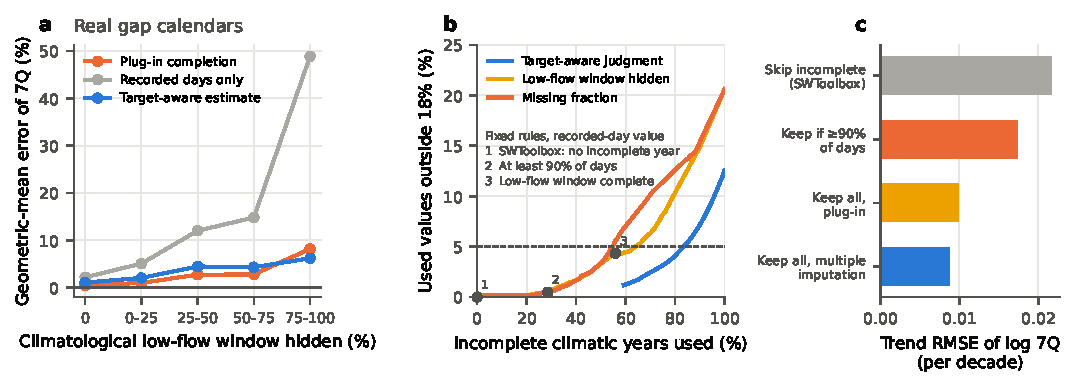
\includegraphics[width=\textwidth]{figures/tr_f7_low_flow.pdf}\caption{Previously opened low-flow illustration, preserved as supplementary context. Its log-flow estimators and incomplete-year practices have their own assumptions and are not the new twenty-seed thermal benchmark.}\end{figure}

Cold-to-hot and calendar splits refit upstream quantities after removing all hot or future years, including from Air2stream, anomaly reference and donor regression training. The annual non-air stress is a deliberately incompatible diagnostic. The separate full daily perturbation adds 0.2$^{\circ}$C per decade to all complete targets and donors and repeats upstream fitting under three seeds. These test different assumptions. Daily-year shifts are applied consistently to complete records and empirical mask calendars.

The Daymet comparison across all 319 USGS source sites changes both spatial product and daily averaging convention. Discharge uses the same original air features with log-flow lags; contradictory daily flow records remain unavailable. All 67,316 original POWER control identities and available points are reproduced exactly. Each alternative has its own shared-case reference. The earlier 35-site standardized-Ridge comparison remains a separate sensitivity. Lags now refer to actual calendar days, including missing leap-year dates, and every unavailable case remains explicit. The prior positional-lag results were reconstructed from the archived script and unchanged cached data; their original output bytes were not retained before overwrite. The European acquisition has \REuropeStations{} usable stations of \REuropeRequested{} requested, and \REuropeCases{} paired cases including \REuropeAirCases{} dangerous air-ridge cases. Nearby GHCN-Daily TAVG matching covers all 319 benchmarkable source USGS sites: 147 have a metadata-eligible station within 25 km, and 122 supply common valid cases. The exact original source control reproduces 67,316 case identities, availability and every available annual point. NOAA daily source S ends at 2400 UTC, while other source conventions vary; this is an observed-input sensitivity, not a perfect riverbank-air or clock-matched oracle. Missing inputs remain in all denominators. Daily metrics use identical dates in both arms. The 7DADM analysis uses approved maxima at 34 sites, without regulatory certification. Historical GAGES-II dam metadata are joined by exact station identifier; zero-flow fractions are proxies and lake-outlet classification is limited to one explicit agency designation. The distance screen fails to flag Big Sandy Creek; observed errors do not determine exclusion.

The selection exercise concerns an assembled panel rather than all USGS sites. Complete-year versus retained-year station eligibility is 98 versus 255 overall and 36 versus 163 in the USGS panel. Same-station slope contrasts, region-group bootstrap intervals, station BH adjustments, synchronized year permutations and circular shifts are reported separately. Estimated incomplete outcomes cannot prove the truth of a changed scientific conclusion. Hot-year hit rates, false alarms and SEDI are preserved even when no valid event denominator exists. The original specification table varies tolerances and decision caps on fixed predictions. A separate twenty-seed, 540-outer-fit H7 pipeline recomputes seven-day peak support, masks, histories, functional draws, MOVE augmentation and annual/risk calibration. Native H7 fields are adapted to the legacy fitting engine after removing the genuine secondary H30 fields; exported native predictions restore H7 names. The daily-input audit reconstructs sixteen provider/tier combinations directly, and default H30 parity passes 240 cases and 201 fields. Deep models and all tolerance/model combinations are not refitted.

Public registration requires platform acceptance and matching protocol/model attachments before any candidate river-temperature observation is requested. Metadata screening of 58 Horizons collection sites finds no candidate with the required four-hot-year calendar support in the current public archive. Screening 218 Greater Wellington catalog sites fixes nine prospective river sites in three conservatively merged management zones. All candidate TimeRange offsets confirm fixed NZST (UTC+12). The frozen primary reference requires complete regular native-day sampling with agency quality code 600; unknown or synthetic quality is excluded. Hourly ERA5-Land air forcing uses the same clock. These rules have synthetic-input tests, but actual reference eligibility remains unverified. The small cohort is a failure-detection design, and ten labeled groups are unavailable by design. E1 and E2 require joint success, with zero admissions and unevaluable groups excluded from passing. No source planning budget reaches 80\% joint success. Public registration and new outcomes are still absent; local files cannot substitute for the platform timestamp. Author and platform fields are reserved for the authors. Release uses the fixed distribution-regression median because that is its classifier's failure target; classical estimation does not inherit that score.

The unflagged-exposure experiment uses the same source cases, masks and true annual targets in both conditions. Seven visible warm days are replaced by concurrent air readings, using air and visibility alone to locate the episode. About 97.6\% of cases support such an episode, with an average 2.3$^{\circ}$C daily air-minus-water shift on replaced days. This is an imposed stress severity, not an estimate of field exposure prevalence. Clean source weights and interval offsets remain fixed; the three seeds vary masks and trajectories. Table~\ref{tab:air-exposure-trends} separates missing-component and total trend coverage, and Table~\ref{tab:air-exposure-release} reports unchanged-score release. Censored trends are omitted here because a contaminated visible window is no longer a valid physical lower bound. Unflagged exposure in an otherwise defined water target must not be interpreted as measurable water temperature in a dry bed.

\begin{figure}[p]\centering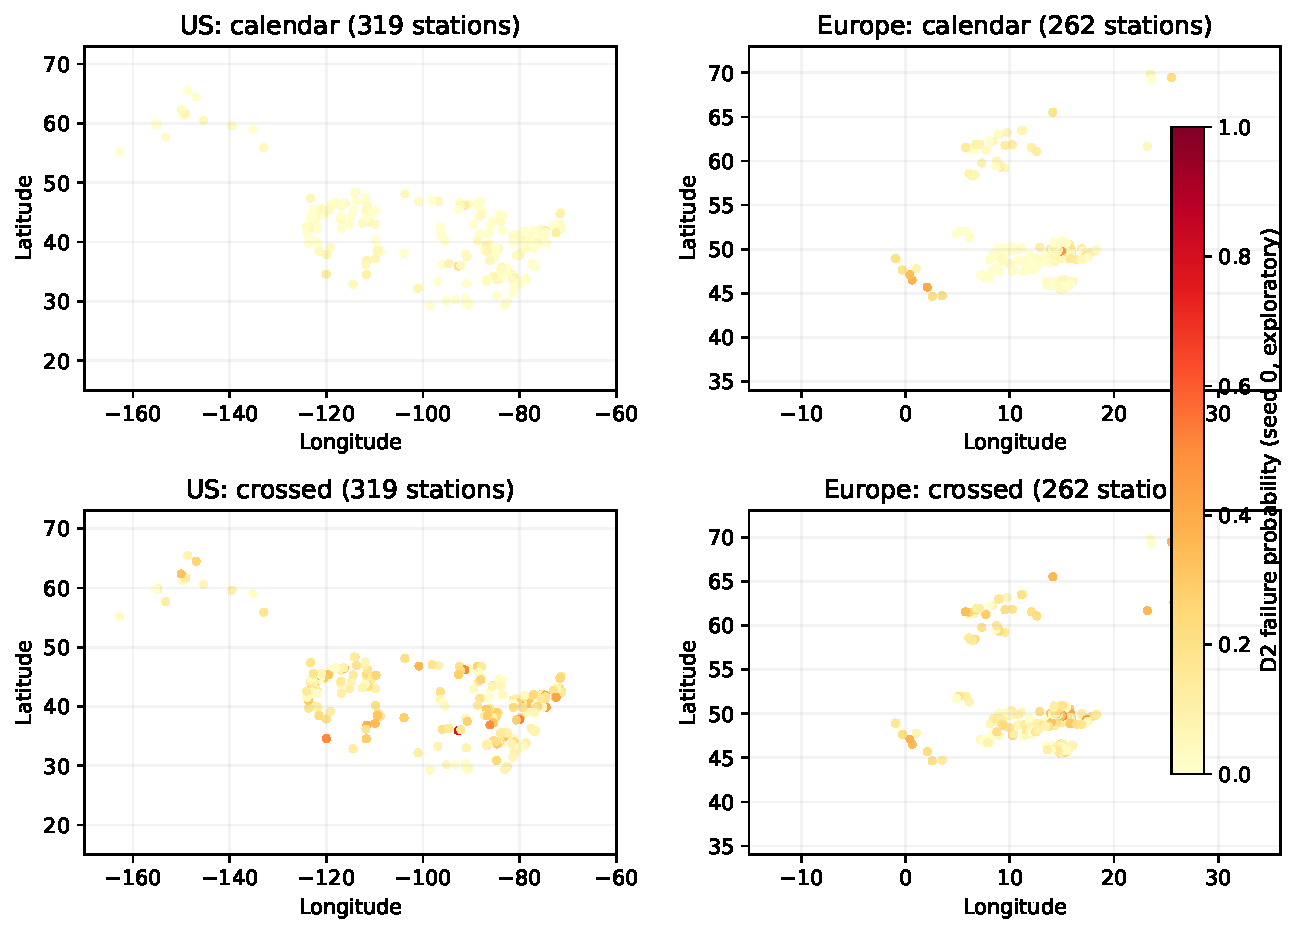
\includegraphics[width=\textwidth]{../../results/wrr_review_completion_20261024/failure_map/failure_map.pdf}\caption{Opened-source station failures and available metadata. Coordinates are available for all 581 stations. The map supports descriptive failure analysis, not causal river-type attribution.}\end{figure}
% DRIVER_RECOVERY_RECOMPUTATION
Forcing-specific recovery probabilities are also recomputed from residual histories excluding both the target year and each residual-validation year. All 269,264 USGS arm/case points reproduce their existing controls, and 1,083 independent daily Ridge checks agree within numerical tolerance. In controlled dangerous air-tier cases, raw Gaussian recovery probabilities average 0.405 against observed failure 0.468 for POWER, and 0.365 against 0.457 for POWER plus flow. These have different available supports and failure targets; they do not establish paired calibration improvement or safe transfer. Complete scores and calibration bins are retained in CSV. Annual distribution and release-classifier weights remain unchanged.

% FOCUSED_STATION_AND_YEAR_DIAGNOSTICS
The two stations specified in the review plan, USGS 13342500 and 06054500, each contribute twenty complete evaluation years; their median shares of random-missingness A1 squared error are 13.0 and 6.1 percent. Historical dam and zero-flow metadata do not identify thermal causation. Named European 2003, 2018 and 2022 examples use common finite cases across all four estimators and preserve event contingency counts, hit/false-alarm rates and undefined SEDI. The 2003 dangerous calendar sample has only 6--22 cases per repetition; median MAE is 0.913 degrees C for D2 and 0.595 for MOVE.1. US illustration years are selected using positive regional air anomalies with at least three complete-water stations, preserving unavailable regions. These opened examples do not establish universal estimator rankings.

% ZERO_FLOW_MISSINGNESS_BOUNDARY
The C1 stratification retains the original 336-USGS-site, 6,479-station-year missingness sample. Approved discharge yields 21 sites with recorded zeros, 266 without a recorded zero and 49 with unavailable flow. A station-conditional logistic model adjusts standardized summer air temperature for linear decade trend; 400 independence-group bootstrap repetitions give OR 1.208 [0.882, 1.564] for the zero-record group and 1.058 [0.988, 1.134] for the available-flow group without recorded zeros. Requiring thirty zero days gives 16 sites and OR 1.282 [0.876, 1.889]. Flow-adjusted specifications have smaller available samples and do not establish mediation. Zero flow is a limited historical proxy, and group exchangeability remains assumed.

The national extension fixes one canonical mean-temperature series per catalog site before numerical analysis, without combining sensors. All 1,273 candidates are attempted; 340 retain unresolved eligibility. National CSVs give eligibility bounds, one-degree station-grid occupancy, HUC2 counts, trends, basin-block stability, BH and synchronized field tests. Hot-year methods share a station threshold from the 90th percentile of at least five complete approved 1981--2010 H30 values; insufficient references remain unavailable. Same-roster/span and common-year comparisons separate added support from changed values. Observed windows provide hot-frequency lower bounds and record witnesses without imputation. Conditional imputation ranges are model sensitivities, not validated confidence coverage.


\begin{table}[p]
\caption{scorecard; source tables contain all strata and empirical repetition intervals.}
\label{tab:scorecard0}
\centering\small
\resizebox{\textwidth}{!}{%
\begin{tabular}{llllll}
\toprule
family & estimator & seeds & MAE & CRPS & coverage \\
\midrule
calendar & H30 MOVE.1 & 20 & 0.992 & -- & -- \\
calendar & Annual MOVE.1 & 20 & 0.550 & -- & -- \\
calendar & Warm-season MOVE.1 & 20 & 0.509 & -- & -- \\
calendar & Air2stream-3 & 20 & 0.568 & -- & -- \\
calendar & Calibrated state & 20 & 0.465 & 0.335 & 0.875 \\
calendar & State simulation & 20 & 0.465 & 0.337 & 0.803 \\
calendar & Distribution regression & 20 & 0.451 & 0.331 & 0.863 \\
calendar & Functional debiasing & 20 & 0.476 & -- & -- \\
calendar & Lookup debiasing & 20 & 0.553 & -- & -- \\
calendar & Observed days & 20 & 4.108 & -- & -- \\
calendar & Daily plug-in & 20 & 0.564 & -- & -- \\
calendar & Stochastic regression & 20 & 0.463 & 0.343 & 0.723 \\
calendar & Calibrated stochastic & 20 & 0.463 & 0.338 & 0.853 \\
calendar & triage\_hybrid & 20 & 0.451 & -- & -- \\
crossed & H30 MOVE.1 & 20 & 1.009 & -- & -- \\
crossed & Annual MOVE.1 & 20 & 0.453 & -- & -- \\
crossed & Warm-season MOVE.1 & 20 & 0.441 & -- & -- \\
crossed & Air2stream-3 & 20 & 0.534 & -- & -- \\
crossed & Calibrated state & 20 & 0.363 & 0.264 & 0.898 \\
crossed & State simulation & 20 & 0.363 & 0.264 & 0.824 \\
\bottomrule
\end{tabular}
}
\end{table}
\begin{table}[p]
\caption{scorecard; source tables contain all strata and empirical repetition intervals.}
\label{tab:scorecard20}
\centering\small
\resizebox{\textwidth}{!}{%
\begin{tabular}{llllll}
\toprule
family & estimator & seeds & MAE & CRPS & coverage \\
\midrule
crossed & Distribution regression & 20 & 0.337 & 0.248 & 0.888 \\
crossed & Functional debiasing & 20 & 0.355 & -- & -- \\
crossed & Lookup debiasing & 20 & 0.422 & -- & -- \\
crossed & Observed days & 20 & 1.427 & -- & -- \\
crossed & Daily plug-in & 20 & 0.428 & -- & -- \\
crossed & Stochastic regression & 20 & 0.336 & 0.248 & 0.753 \\
crossed & Calibrated stochastic & 20 & 0.337 & 0.247 & 0.892 \\
crossed & triage\_hybrid & 20 & 0.337 & -- & -- \\
\bottomrule
\end{tabular}
}
\end{table}
\begin{table}[p]
\caption{rules; source tables contain all strata and empirical repetition intervals.}
\label{tab:rules0}
\centering\small
\resizebox{\textwidth}{!}{%
\begin{tabular}{lllllll}
\toprule
family & delivery & rule & seeds & retention & risk & groups \(>\)10\% \\
\midrule
calendar & Distribution regression & all & 20 & 1.000 & 0.030 & 0.071 \\
calendar & Distribution regression & atc & 20 & 0.965 & 0.014 & 0.006 \\
calendar & Distribution regression & Batch average & 20 & 0.994 & 0.027 & 0.033 \\
calendar & Distribution regression & Batch + individual cap & 20 & 0.966 & 0.014 & 0.011 \\
calendar & Distribution regression & gap\_49 & 20 & 0.806 & 0.005 & 0.000 \\
calendar & Distribution regression & Group certificate & 20 & 0.000 & -- & -- \\
calendar & Distribution regression & individual\_0.05 & 20 & 0.938 & 0.005 & 0.000 \\
calendar & Distribution regression & Individual score \(\leq\)0.10 & 20 & 0.948 & 0.008 & 0.000 \\
calendar & Distribution regression & individual\_0.2 & 20 & 0.959 & 0.011 & 0.006 \\
calendar & Distribution regression & individual\_0.3 & 20 & 0.967 & 0.014 & 0.011 \\
calendar & Distribution regression & Probability + group adjustment & 20 & 0.921 & 0.003 & 0.000 \\
calendar & Distribution regression & mondrian & 20 & 0.966 & 0.014 & 0.011 \\
calendar & Distribution regression & none & 20 & 0.000 & -- & -- \\
calendar & Distribution regression & one\_feature\_25 & 20 & 0.889 & 0.003 & 0.000 \\
calendar & Distribution regression & Peak overlap \(<\)50\% & 20 & 0.916 & 0.005 & 0.000 \\
calendar & Distribution regression & published\_Beaufort\_full & 20 & 0.645 & 0.001 & 0.000 \\
calendar & Distribution regression & published\_Beaufort\_full\_as\_written & 20 & 0.641 & 0.001 & 0.000 \\
calendar & Distribution regression & published\_Dunham\_full & 20 & 0.654 & 0.002 & 0.000 \\
calendar & Distribution regression & published\_Dunham\_full\_as\_written & 20 & 0.655 & 0.002 & 0.000 \\
calendar & Distribution regression & published\_ETCCDI\_15\_3 & 20 & 0.350 & 0.000 & 0.000 \\
\bottomrule
\end{tabular}
}
\end{table}
\begin{table}[p]
\caption{rules; source tables contain all strata and empirical repetition intervals.}
\label{tab:rules20}
\centering\small
\resizebox{\textwidth}{!}{%
\begin{tabular}{lllllll}
\toprule
family & delivery & rule & seeds & retention & risk & groups \(>\)10\% \\
\midrule
calendar & Distribution regression & published\_GSIM\_350 & 20 & 0.590 & 0.000 & 0.000 \\
calendar & Distribution regression & published\_NorWest90 & 20 & 0.847 & 0.004 & 0.000 \\
calendar & Distribution regression & published\_NorWest90\_as\_written & 20 & 0.848 & 0.004 & 0.000 \\
calendar & Distribution regression & published\_Oregon80 & 20 & 0.873 & 0.003 & 0.000 \\
calendar & Distribution regression & published\_Oregon80\_as\_written & 20 & 0.875 & 0.003 & 0.000 \\
calendar & Distribution regression & published\_USGS\_311\_24 & 20 & 0.517 & 0.000 & 0.000 \\
calendar & Distribution regression & published\_USGS\_strict7 & 20 & 0.167 & 0.000 & 0.000 \\
calendar & Distribution regression & published\_WMO\_11\_5 & 20 & 0.432 & 0.000 & 0.000 \\
calendar & Distribution regression & published\_complete\_year & 20 & 0.000 & -- & -- \\
calendar & Distribution regression & published\_gap14 & 20 & 0.648 & 0.001 & 0.000 \\
calendar & Distribution regression & published\_gap49 & 20 & 0.806 & 0.005 & 0.000 \\
calendar & Distribution regression & published\_warm\_gap14 & 20 & 0.813 & 0.001 & 0.000 \\
calendar & Distribution regression & published\_warm\_gap30 & 20 & 0.885 & 0.003 & 0.000 \\
calendar & Distribution regression & published\_warm\_gap7 & 20 & 0.745 & 0.000 & 0.000 \\
calendar & Distribution regression & random\_effects & 20 & 0.000 & 0.003 & 0.000 \\
calendar & Distribution regression & 90\% warm-season coverage & 20 & 0.789 & 0.000 & 0.000 \\
calendar & Observed days & one\_feature\_25 & 20 & 0.889 & 0.009 & 0.000 \\
calendar & Observed days & Peak overlap \(<\)50\% & 20 & 0.916 & 0.018 & 0.000 \\
calendar & Observed days & published\_Beaufort\_full & 20 & 0.645 & 0.001 & 0.000 \\
calendar & Observed days & published\_Beaufort\_full\_as\_written & 20 & 0.641 & 0.002 & 0.000 \\
\bottomrule
\end{tabular}
}
\end{table}
\begin{table}[p]
\caption{rules; source tables contain all strata and empirical repetition intervals.}
\label{tab:rules40}
\centering\small
\resizebox{\textwidth}{!}{%
\begin{tabular}{lllllll}
\toprule
family & delivery & rule & seeds & retention & risk & groups \(>\)10\% \\
\midrule
calendar & Observed days & published\_Dunham\_full & 20 & 0.654 & 0.004 & 0.000 \\
calendar & Observed days & published\_Dunham\_full\_as\_written & 20 & 0.655 & 0.004 & 0.000 \\
calendar & Observed days & published\_ETCCDI\_15\_3 & 20 & 0.350 & 0.000 & 0.000 \\
calendar & Observed days & published\_GSIM\_350 & 20 & 0.590 & 0.003 & 0.000 \\
calendar & Observed days & published\_NorWest90 & 20 & 0.847 & 0.011 & 0.000 \\
calendar & Observed days & published\_NorWest90\_as\_written & 20 & 0.848 & 0.012 & 0.000 \\
calendar & Observed days & published\_Oregon80 & 20 & 0.873 & 0.010 & 0.000 \\
calendar & Observed days & published\_Oregon80\_as\_written & 20 & 0.875 & 0.010 & 0.000 \\
calendar & Observed days & published\_USGS\_311\_24 & 20 & 0.517 & 0.001 & 0.000 \\
calendar & Observed days & published\_USGS\_strict7 & 20 & 0.167 & 0.000 & 0.000 \\
calendar & Observed days & published\_WMO\_11\_5 & 20 & 0.432 & 0.000 & 0.000 \\
calendar & Observed days & published\_complete\_year & 20 & 0.000 & -- & -- \\
calendar & Observed days & published\_gap14 & 20 & 0.648 & 0.009 & 0.000 \\
calendar & Observed days & published\_gap49 & 20 & 0.806 & 0.025 & 0.000 \\
calendar & Observed days & published\_warm\_gap14 & 20 & 0.813 & 0.008 & 0.000 \\
calendar & Observed days & published\_warm\_gap30 & 20 & 0.885 & 0.018 & 0.000 \\
calendar & Observed days & published\_warm\_gap7 & 20 & 0.745 & 0.002 & 0.000 \\
calendar & Daily plug-in & one\_feature\_25 & 20 & 0.889 & 0.005 & 0.000 \\
calendar & Daily plug-in & Peak overlap \(<\)50\% & 20 & 0.916 & 0.008 & 0.000 \\
calendar & Daily plug-in & published\_Beaufort\_full & 20 & 0.645 & 0.001 & 0.000 \\
\bottomrule
\end{tabular}
}
\end{table}
\begin{table}[p]
\caption{rules; source tables contain all strata and empirical repetition intervals.}
\label{tab:rules60}
\centering\small
\resizebox{\textwidth}{!}{%
\begin{tabular}{lllllll}
\toprule
family & delivery & rule & seeds & retention & risk & groups \(>\)10\% \\
\midrule
calendar & Daily plug-in & published\_Beaufort\_full\_as\_written & 20 & 0.641 & 0.002 & 0.000 \\
calendar & Daily plug-in & published\_Dunham\_full & 20 & 0.654 & 0.003 & 0.000 \\
calendar & Daily plug-in & published\_Dunham\_full\_as\_written & 20 & 0.655 & 0.003 & 0.000 \\
calendar & Daily plug-in & published\_ETCCDI\_15\_3 & 20 & 0.350 & 0.000 & 0.000 \\
calendar & Daily plug-in & published\_GSIM\_350 & 20 & 0.590 & 0.001 & 0.000 \\
calendar & Daily plug-in & published\_NorWest90 & 20 & 0.847 & 0.006 & 0.000 \\
calendar & Daily plug-in & published\_NorWest90\_as\_written & 20 & 0.848 & 0.007 & 0.000 \\
calendar & Daily plug-in & published\_Oregon80 & 20 & 0.873 & 0.005 & 0.000 \\
calendar & Daily plug-in & published\_Oregon80\_as\_written & 20 & 0.875 & 0.005 & 0.000 \\
calendar & Daily plug-in & published\_USGS\_311\_24 & 20 & 0.517 & 0.001 & 0.000 \\
calendar & Daily plug-in & published\_USGS\_strict7 & 20 & 0.167 & 0.000 & 0.000 \\
calendar & Daily plug-in & published\_WMO\_11\_5 & 20 & 0.432 & 0.000 & 0.000 \\
calendar & Daily plug-in & published\_complete\_year & 20 & 0.000 & -- & -- \\
calendar & Daily plug-in & published\_gap14 & 20 & 0.648 & 0.003 & 0.000 \\
calendar & Daily plug-in & published\_gap49 & 20 & 0.806 & 0.010 & 0.000 \\
calendar & Daily plug-in & published\_warm\_gap14 & 20 & 0.813 & 0.003 & 0.000 \\
calendar & Daily plug-in & published\_warm\_gap30 & 20 & 0.885 & 0.007 & 0.000 \\
calendar & Daily plug-in & published\_warm\_gap7 & 20 & 0.745 & 0.001 & 0.000 \\
crossed & Distribution regression & all & 20 & 1.000 & 0.126 & 0.662 \\
crossed & Distribution regression & atc & 20 & 0.861 & 0.078 & 0.384 \\
\bottomrule
\end{tabular}
}
\end{table}
\begin{table}[p]
\caption{rules; source tables contain all strata and empirical repetition intervals.}
\label{tab:rules80}
\centering\small
\resizebox{\textwidth}{!}{%
\begin{tabular}{lllllll}
\toprule
family & delivery & rule & seeds & retention & risk & groups \(>\)10\% \\
\midrule
crossed & Distribution regression & Batch average & 20 & 0.858 & 0.078 & 0.368 \\
crossed & Distribution regression & Batch + individual cap & 20 & 0.847 & 0.074 & 0.346 \\
crossed & Distribution regression & gap\_49 & 20 & 0.333 & 0.082 & 0.400 \\
crossed & Distribution regression & Group certificate & 20 & 0.000 & -- & -- \\
crossed & Distribution regression & individual\_0.05 & 20 & 0.708 & 0.038 & 0.068 \\
crossed & Distribution regression & Individual score \(\leq\)0.10 & 20 & 0.768 & 0.052 & 0.149 \\
crossed & Distribution regression & individual\_0.2 & 20 & 0.832 & 0.070 & 0.303 \\
crossed & Distribution regression & individual\_0.3 & 20 & 0.871 & 0.081 & 0.405 \\
crossed & Distribution regression & Probability + group adjustment & 20 & 0.618 & 0.021 & 0.027 \\
crossed & Distribution regression & mondrian & 20 & 0.841 & 0.072 & 0.311 \\
crossed & Distribution regression & none & 20 & 0.000 & -- & -- \\
crossed & Distribution regression & one\_feature\_25 & 20 & 0.381 & 0.015 & 0.014 \\
crossed & Distribution regression & Peak overlap \(<\)50\% & 20 & 0.492 & 0.035 & 0.043 \\
crossed & Distribution regression & published\_Beaufort\_full & 20 & 0.281 & 0.003 & 0.005 \\
crossed & Distribution regression & published\_Beaufort\_full\_as\_written & 20 & 0.291 & 0.013 & 0.030 \\
crossed & Distribution regression & published\_Dunham\_full & 20 & 0.281 & 0.007 & 0.006 \\
crossed & Distribution regression & published\_Dunham\_full\_as\_written & 20 & 0.292 & 0.011 & 0.011 \\
crossed & Distribution regression & published\_ETCCDI\_15\_3 & 20 & 0.000 & -- & -- \\
crossed & Distribution regression & published\_GSIM\_350 & 20 & 0.000 & -- & -- \\
crossed & Distribution regression & published\_NorWest90 & 20 & 0.436 & 0.042 & 0.086 \\
\bottomrule
\end{tabular}
}
\end{table}
\begin{table}[p]
\caption{rules; source tables contain all strata and empirical repetition intervals.}
\label{tab:rules100}
\centering\small
\resizebox{\textwidth}{!}{%
\begin{tabular}{lllllll}
\toprule
family & delivery & rule & seeds & retention & risk & groups \(>\)10\% \\
\midrule
crossed & Distribution regression & published\_NorWest90\_as\_written & 20 & 0.442 & 0.043 & 0.114 \\
crossed & Distribution regression & published\_Oregon80 & 20 & 0.285 & 0.006 & 0.005 \\
crossed & Distribution regression & published\_Oregon80\_as\_written & 20 & 0.313 & 0.015 & 0.022 \\
crossed & Distribution regression & published\_USGS\_311\_24 & 20 & 0.000 & -- & -- \\
crossed & Distribution regression & published\_USGS\_strict7 & 20 & 0.000 & -- & -- \\
crossed & Distribution regression & published\_WMO\_11\_5 & 20 & 0.000 & -- & -- \\
crossed & Distribution regression & published\_complete\_year & 20 & 0.000 & -- & -- \\
crossed & Distribution regression & published\_gap14 & 20 & 0.000 & -- & -- \\
crossed & Distribution regression & published\_gap49 & 20 & 0.333 & 0.082 & 0.400 \\
crossed & Distribution regression & published\_warm\_gap14 & 20 & 0.181 & 0.001 & 0.006 \\
crossed & Distribution regression & published\_warm\_gap30 & 20 & 0.478 & 0.058 & 0.238 \\
crossed & Distribution regression & published\_warm\_gap7 & 20 & 0.159 & 0.001 & 0.000 \\
crossed & Distribution regression & random\_effects & 20 & 0.000 & 0.000 & 0.000 \\
crossed & Distribution regression & 90\% warm-season coverage & 20 & 0.184 & 0.001 & 0.006 \\
crossed & Observed days & one\_feature\_25 & 20 & 0.381 & 0.038 & 0.024 \\
crossed & Observed days & Peak overlap \(<\)50\% & 20 & 0.492 & 0.097 & 0.397 \\
crossed & Observed days & published\_Beaufort\_full & 20 & 0.281 & 0.005 & 0.000 \\
crossed & Observed days & published\_Beaufort\_full\_as\_written & 20 & 0.291 & 0.022 & 0.044 \\
crossed & Observed days & published\_Dunham\_full & 20 & 0.281 & 0.013 & 0.000 \\
crossed & Observed days & published\_Dunham\_full\_as\_written & 20 & 0.292 & 0.024 & 0.039 \\
\bottomrule
\end{tabular}
}
\end{table}
\begin{table}[p]
\caption{rules; source tables contain all strata and empirical repetition intervals.}
\label{tab:rules120}
\centering\small
\resizebox{\textwidth}{!}{%
\begin{tabular}{lllllll}
\toprule
family & delivery & rule & seeds & retention & risk & groups \(>\)10\% \\
\midrule
crossed & Observed days & published\_ETCCDI\_15\_3 & 20 & 0.000 & -- & -- \\
crossed & Observed days & published\_GSIM\_350 & 20 & 0.000 & -- & -- \\
crossed & Observed days & published\_NorWest90 & 20 & 0.436 & 0.114 & 0.557 \\
crossed & Observed days & published\_NorWest90\_as\_written & 20 & 0.442 & 0.121 & 0.595 \\
crossed & Observed days & published\_Oregon80 & 20 & 0.285 & 0.013 & 0.000 \\
crossed & Observed days & published\_Oregon80\_as\_written & 20 & 0.313 & 0.034 & 0.070 \\
crossed & Observed days & published\_USGS\_311\_24 & 20 & 0.000 & -- & -- \\
crossed & Observed days & published\_USGS\_strict7 & 20 & 0.000 & -- & -- \\
crossed & Observed days & published\_WMO\_11\_5 & 20 & 0.000 & -- & -- \\
crossed & Observed days & published\_complete\_year & 20 & 0.000 & -- & -- \\
crossed & Observed days & published\_gap14 & 20 & 0.000 & -- & -- \\
crossed & Observed days & published\_gap49 & 20 & 0.333 & 0.305 & 0.984 \\
crossed & Observed days & published\_warm\_gap14 & 20 & 0.181 & 0.000 & 0.003 \\
crossed & Observed days & published\_warm\_gap30 & 20 & 0.478 & 0.213 & 0.962 \\
crossed & Observed days & published\_warm\_gap7 & 20 & 0.159 & 0.000 & 0.000 \\
crossed & Daily plug-in & one\_feature\_25 & 20 & 0.381 & 0.021 & 0.022 \\
crossed & Daily plug-in & Peak overlap \(<\)50\% & 20 & 0.492 & 0.049 & 0.141 \\
crossed & Daily plug-in & published\_Beaufort\_full & 20 & 0.281 & 0.004 & 0.006 \\
crossed & Daily plug-in & published\_Beaufort\_full\_as\_written & 20 & 0.291 & 0.017 & 0.049 \\
crossed & Daily plug-in & published\_Dunham\_full & 20 & 0.281 & 0.008 & 0.008 \\
\bottomrule
\end{tabular}
}
\end{table}
\begin{table}[p]
\caption{rules; source tables contain all strata and empirical repetition intervals.}
\label{tab:rules140}
\centering\small
\resizebox{\textwidth}{!}{%
\begin{tabular}{lllllll}
\toprule
family & delivery & rule & seeds & retention & risk & groups \(>\)10\% \\
\midrule
crossed & Daily plug-in & published\_Dunham\_full\_as\_written & 20 & 0.292 & 0.015 & 0.033 \\
crossed & Daily plug-in & published\_ETCCDI\_15\_3 & 20 & 0.000 & -- & -- \\
crossed & Daily plug-in & published\_GSIM\_350 & 20 & 0.000 & -- & -- \\
crossed & Daily plug-in & published\_NorWest90 & 20 & 0.436 & 0.057 & 0.200 \\
crossed & Daily plug-in & published\_NorWest90\_as\_written & 20 & 0.442 & 0.059 & 0.232 \\
crossed & Daily plug-in & published\_Oregon80 & 20 & 0.285 & 0.008 & 0.011 \\
crossed & Daily plug-in & published\_Oregon80\_as\_written & 20 & 0.313 & 0.020 & 0.043 \\
crossed & Daily plug-in & published\_USGS\_311\_24 & 20 & 0.000 & -- & -- \\
crossed & Daily plug-in & published\_USGS\_strict7 & 20 & 0.000 & -- & -- \\
crossed & Daily plug-in & published\_WMO\_11\_5 & 20 & 0.000 & -- & -- \\
crossed & Daily plug-in & published\_complete\_year & 20 & 0.000 & -- & -- \\
crossed & Daily plug-in & published\_gap14 & 20 & 0.000 & -- & -- \\
crossed & Daily plug-in & published\_gap49 & 20 & 0.333 & 0.127 & 0.641 \\
crossed & Daily plug-in & published\_warm\_gap14 & 20 & 0.181 & 0.001 & 0.006 \\
crossed & Daily plug-in & published\_warm\_gap30 & 20 & 0.478 & 0.089 & 0.454 \\
crossed & Daily plug-in & published\_warm\_gap7 & 20 & 0.159 & 0.001 & 0.000 \\
\bottomrule
\end{tabular}
}
\end{table}
\begin{table}[p]
\caption{recovery; source tables contain all strata and empirical repetition intervals.}
\label{tab:recovery0}
\centering\small
\resizebox{\textwidth}{!}{%
\begin{tabular}{lllll}
\toprule
family & scope & model & seeds & auc median \\
\midrule
calendar & all & lookup & 20 & 0.921 \\
calendar & all & one\_feature & 20 & 0.933 \\
calendar & all & oracle\_D2 & 20 & 1.000 \\
calendar & all & oracle\_plugin & 20 & 1.000 \\
calendar & all & recovery\_model & 20 & 0.972 \\
calendar & all & recovery\_t5 & 20 & 0.969 \\
calendar & all & risk\_classifier & 20 & 0.978 \\
calendar & danger & lookup & 20 & 0.643 \\
calendar & danger & one\_feature & 20 & 0.615 \\
calendar & danger & oracle\_D2 & 20 & 1.000 \\
calendar & danger & oracle\_plugin & 20 & 1.000 \\
calendar & danger & recovery\_model & 20 & 0.780 \\
calendar & danger & recovery\_t5 & 20 & 0.767 \\
calendar & danger & risk\_classifier & 20 & 0.751 \\
calendar & within\_cell & recovery\_model & 20 & 0.873 \\
crossed & all & lookup & 20 & 0.785 \\
crossed & all & one\_feature & 20 & 0.756 \\
crossed & all & oracle\_D2 & 20 & 1.000 \\
crossed & all & oracle\_plugin & 20 & 1.000 \\
crossed & all & recovery\_model & 20 & 0.867 \\
\bottomrule
\end{tabular}
}
\end{table}
\begin{table}[p]
\caption{recovery; source tables contain all strata and empirical repetition intervals.}
\label{tab:recovery20}
\centering\small
\resizebox{\textwidth}{!}{%
\begin{tabular}{lllll}
\toprule
family & scope & model & seeds & auc median \\
\midrule
crossed & all & recovery\_t5 & 20 & 0.856 \\
crossed & all & risk\_classifier & 20 & 0.866 \\
crossed & danger & lookup & 20 & 0.635 \\
crossed & danger & one\_feature & 20 & 0.557 \\
crossed & danger & oracle\_D2 & 20 & 1.000 \\
crossed & danger & oracle\_plugin & 20 & 1.000 \\
crossed & danger & recovery\_model & 20 & 0.784 \\
crossed & danger & recovery\_t5 & 20 & 0.771 \\
crossed & danger & risk\_classifier & 20 & 0.763 \\
crossed & within\_cell & recovery\_model & 20 & 0.806 \\
\bottomrule
\end{tabular}
}
\end{table}
\begin{table}[p]
\caption{Matched deep-comparator crossed cases with dangerous gaps and air-ridge information tier; three seeds only. Neighbor data are absent from neural inputs.}
\label{tab:deepcrossed}
\centering\small
\resizebox{\textwidth}{!}{%
\begin{tabular}{lllll}
\toprule
model & seeds & MAE & bias median & availability median \\
\midrule
boosting & 3 & 0.556 & 0.008 & 1.000 \\
Global lagged-air boosting & 3 & 0.490 & 0.105 & 1.000 \\
Local air boosting & 3 & 0.447 & 0.097 & 1.000 \\
Local flow boosting & 3 & 0.398 & 0.129 & 0.600 \\
Global flow boosting & 3 & 0.579 & 0.257 & 0.600 \\
CSDI & 3 & 0.531 & -0.010 & 1.000 \\
distribution\_regression\_calibrated & 3 & 0.333 & 0.155 & 1.000 \\
distribution\_regression\_raw & 3 & 0.333 & 0.155 & 1.000 \\
Functional debiasing & 3 & 0.338 & 0.133 & 1.000 \\
LSTM & 3 & 0.479 & 0.135 & 1.000 \\
SAITS & 3 & 0.460 & -0.003 & 1.000 \\
stochastic\_regression\_calibrated\_local & 3 & 0.261 & -0.065 & 1.000 \\
stochastic\_regression\_local & 3 & 0.261 & -0.065 & 1.000 \\
\bottomrule
\end{tabular}
}
\end{table}
\begin{table}[p]
\caption{Matched deep-comparator calendar cases with dangerous gaps and air-ridge information tier; three seeds only. Neighbor data are absent from neural inputs.}
\label{tab:deepcalendar}
\centering\small
\resizebox{\textwidth}{!}{%
\begin{tabular}{lllll}
\toprule
model & seeds & MAE & bias median & availability median \\
\midrule
boosting & 3 & 0.793 & -0.397 & 1.000 \\
Global lagged-air boosting & 3 & 0.699 & -0.045 & 1.000 \\
Local air boosting & 3 & 0.643 & -0.320 & 1.000 \\
Local flow boosting & 3 & 0.345 & -0.065 & 0.429 \\
Global flow boosting & 3 & 0.620 & -0.281 & 0.429 \\
CSDI & 3 & 0.689 & -0.304 & 1.000 \\
distribution\_regression\_calibrated & 3 & 0.470 & 0.069 & 1.000 \\
distribution\_regression\_raw & 3 & 0.470 & 0.069 & 1.000 \\
Functional debiasing & 3 & 0.524 & 0.134 & 1.000 \\
LSTM & 3 & 0.697 & -0.083 & 1.000 \\
SAITS & 3 & 0.825 & -0.518 & 1.000 \\
stochastic\_regression\_calibrated\_local & 3 & 0.894 & -0.526 & 1.000 \\
stochastic\_regression\_local & 3 & 0.894 & -0.526 & 1.000 \\
\bottomrule
\end{tabular}
}
\end{table}
\begin{table}[p]
\caption{Nonempty bounded-group certification by local label budget. Undefined selected risks are not zero-risk successes.}
\label{tab:local-labels}
\centering\small
\resizebox{\textwidth}{!}{%
\begin{tabular}{llllll}
\toprule
family & labels (groups) & runs & nonempty certificate fraction & mean retention & risk among nonempty \\
\midrule
calendar & 2 & 40000 & 0.000 & 0.000 & -- \\
calendar & 4 & 28000 & 0.000 & 0.000 & -- \\
calendar & 8 & 18000 & 0.000 & 0.000 & -- \\
calendar & 10 & 14000 & 0.000 & 0.000 & -- \\
calendar & 16 & 6000 & 0.000 & 0.000 & -- \\
crossed & 2 & 40000 & 0.000 & 0.000 & -- \\
crossed & 4 & 28000 & 0.000 & 0.000 & -- \\
crossed & 8 & 18000 & 0.000 & 0.000 & -- \\
crossed & 10 & 14000 & 0.000 & 0.000 & -- \\
crossed & 16 & 6000 & 0.000 & 0.000 & -- \\
\bottomrule
\end{tabular}
}
\end{table}
\begin{table}[p]
\caption{Poststratified outcomes per 1,000 historically supported incomplete station-years. Empirical repetition medians; unsupported strata stay in the denominator.}
\label{tab:per1000}
\centering\small
\resizebox{\textwidth}{!}{%
\begin{tabular}{llll}
\toprule
rule & used per 1000 median & failures per 1000 median & unsupported population per 1000 median \\
\midrule
all & 997.162 & 28.588 & 2.838 \\
individual\_0.05 & 933.980 & 3.997 & 2.838 \\
Individual score \(\leq\)0.10 & 942.808 & 5.769 & 2.838 \\
individual\_0.2 & 953.531 & 9.070 & 2.838 \\
individual\_0.3 & 961.355 & 11.766 & 2.838 \\
one\_feature\_25 & 893.668 & 2.913 & 2.838 \\
Peak overlap \(<\)50\% & 924.923 & 4.721 & 2.838 \\
warm90 & 799.642 & 0.583 & 2.838 \\
\bottomrule
\end{tabular}
}
\end{table}
\begin{table}[p]
\caption{Exact frozen-admission deletion sensitivity. The best published comparator is fixed using opened full-data outcomes at a 5 percent point-risk cap. A zero is an initial failure; unavailable reversal minima remain undefined.}
\label{tab:group-deletions}
\centering\small
\resizebox{\textwidth}{!}{%
\begin{tabular}{llllll}
\toprule
family & rule & repeats & finite minima & initial failures & median min. groups \\
\midrule
calendar & Batch average & 20 & 20 & 0 & 179.500 \\
calendar & Batch + individual cap & 20 & 20 & 0 & 168.500 \\
calendar & Individual score \(\leq\)0.10 & 20 & 20 & 0 & 150.500 \\
calendar & Probability + group adjustment & 20 & 20 & 0 & 87.000 \\
crossed & Batch average & 20 & 20 & 20 & 0.000 \\
crossed & Batch + individual cap & 20 & 20 & 20 & 0.000 \\
crossed & Individual score \(\leq\)0.10 & 20 & 19 & 15 & 0.000 \\
crossed & Probability + group adjustment & 20 & 20 & 0 & 114.000 \\
\bottomrule
\end{tabular}
}
\end{table}
\begin{table}[p]
\caption{Historical opened N1 uses a 7 percent point-risk criterion. Fixed-admission minima and batch-rule reapplication at the witness answer different questions; historical verdicts do not change.}
\label{tab:historical-n1-deletion}
\centering\small
\resizebox{\textwidth}{!}{%
\begin{tabular}{lllll}
\toprule
population & n groups & minimum groups & remaining risk & reapplied witness risk \\
\midrule
deploy & 40 & 10 & 0.071 & 0.056 \\
mech & 40 & 10 & 0.071 & 0.062 \\
\bottomrule
\end{tabular}
}
\end{table}
\begin{table}[p]
\caption{Conditional conformal prediction-set comparators over twenty seeds. Conditional coverage targets false-admission frequency per eligible representative, not selected risk. Region means are descriptive under held-region shift; empty releases have undefined selected risk.}
\label{tab:formal-conditional}
\centering\small
\resizebox{\textwidth}{!}{%
\begin{tabular}{llllllll}
\toprule
family & method & nominal coverage & seeds & retention & coverage & selected risk & LP fallback (\%) \\
\midrule
calendar & Coarse groups, conservative & 0.900 & 20 & 0.000 & 1.000 & -- & 0.000 \\
calendar & Coarse groups, conservative & 0.950 & 20 & 0.000 & 1.000 & -- & 0.000 \\
calendar & Coarse groups, randomized & 0.900 & 20 & 0.156 & 0.900 & 0.005 & 1.754 \\
calendar & Coarse groups, randomized & 0.950 & 20 & 0.078 & 0.950 & 0.005 & 0.962 \\
calendar & Full region, randomized & 0.900 & 20 & 0.000 & 0.901 & -- & 0.000 \\
calendar & Full region, randomized & 0.950 & 20 & 0.000 & 0.950 & -- & 0.000 \\
calendar & Full region, conservative & 0.900 & 20 & 0.000 & 1.000 & -- & 0.000 \\
calendar & Full region, conservative & 0.950 & 20 & 0.000 & 1.000 & -- & 0.000 \\
crossed & Coarse groups, conservative & 0.900 & 20 & 0.000 & 1.000 & -- & 0.000 \\
crossed & Coarse groups, conservative & 0.950 & 20 & 0.000 & 1.000 & -- & 0.000 \\
crossed & Coarse groups, randomized & 0.900 & 20 & 0.111 & 0.900 & 0.083 & 0.824 \\
crossed & Coarse groups, randomized & 0.950 & 20 & 0.055 & 0.950 & 0.086 & 0.510 \\
crossed & Full region, randomized & 0.900 & 20 & 0.000 & 0.900 & -- & 0.000 \\
crossed & Full region, randomized & 0.950 & 20 & 0.000 & 0.950 & -- & 0.000 \\
crossed & Full region, conservative & 0.900 & 20 & 0.000 & 1.000 & -- & 0.000 \\
crossed & Full region, conservative & 0.950 & 20 & 0.000 & 1.000 & -- & 0.000 \\
\bottomrule
\end{tabular}
}
\end{table}
\begin{table}[p]
\caption{Identical classifier and cap: isolate Platt probability calibration from its additional empirical overlapping-group factors. These are exploratory source repetition medians, not the formal conditional-conformal algorithm.}
\label{tab:probability-ablation}
\centering\small
\resizebox{\textwidth}{!}{%
\begin{tabular}{llllll}
\toprule
family & method & retention & risk & fraction groups above 10 & worst group risk \\
\midrule
calendar & Probability + group adjustment & 0.921 & 0.003 & 0.000 & 0.045 \\
calendar & Platt probability calibration & 0.925 & 0.003 & 0.000 & 0.047 \\
calendar & Raw classifier & 0.948 & 0.008 & 0.000 & 0.080 \\
crossed & Probability + group adjustment & 0.618 & 0.021 & 0.027 & 0.159 \\
crossed & Platt probability calibration & 0.638 & 0.024 & 0.032 & 0.170 \\
crossed & Raw classifier & 0.768 & 0.052 & 0.149 & 0.231 \\
\bottomrule
\end{tabular}
}
\end{table}
\begin{table}[p]
\caption{General-loss semi-supervised and labeled-only RCPS with WSR bounds. The unit is an independent group. Distinct unlabeled calibration groups and untouched test groups are required.}
\label{tab:formal-semicalendar}
\centering\small
\resizebox{\textwidth}{!}{%
\begin{tabular}{lllll}
\toprule
method & labels (groups) & runs & nonempty & unlabeled shortage \\
\midrule
Labeled-only WSR & 2 & 40000 & 0.000 & 0.000 \\
Labeled-only WSR & 4 & 28000 & 0.000 & 0.000 \\
Labeled-only WSR & 8 & 18000 & 0.000 & 0.000 \\
Labeled-only WSR & 10 & 14000 & 0.000 & 0.000 \\
Labeled-only WSR & 16 & 6000 & 0.000 & 0.000 \\
Semi-supervised WSR & 2 & 40000 & 0.000 & 0.400 \\
Semi-supervised WSR & 4 & 28000 & 0.000 & 0.643 \\
Semi-supervised WSR & 8 & 18000 & 0.000 & 1.000 \\
Semi-supervised WSR & 10 & 14000 & 0.000 & 1.000 \\
Semi-supervised WSR & 16 & 6000 & 0.000 & 1.000 \\
\bottomrule
\end{tabular}
}
\end{table}
\begin{table}[p]
\caption{General-loss semi-supervised and labeled-only RCPS with WSR bounds. The unit is an independent group. Distinct unlabeled calibration groups and untouched test groups are required.}
\label{tab:formal-semicrossed}
\centering\small
\resizebox{\textwidth}{!}{%
\begin{tabular}{lllll}
\toprule
method & labels (groups) & runs & nonempty & unlabeled shortage \\
\midrule
Labeled-only WSR & 2 & 40000 & 0.000 & 0.000 \\
Labeled-only WSR & 4 & 28000 & 0.000 & 0.000 \\
Labeled-only WSR & 8 & 18000 & 0.000 & 0.000 \\
Labeled-only WSR & 10 & 14000 & 0.000 & 0.000 \\
Labeled-only WSR & 16 & 6000 & 0.000 & 0.000 \\
Semi-supervised WSR & 2 & 40000 & 0.000 & 0.400 \\
Semi-supervised WSR & 4 & 28000 & 0.000 & 0.643 \\
Semi-supervised WSR & 8 & 18000 & 0.000 & 1.000 \\
Semi-supervised WSR & 10 & 14000 & 0.000 & 1.000 \\
Semi-supervised WSR & 16 & 6000 & 0.000 & 1.000 \\
\bottomrule
\end{tabular}
}
\end{table}
\begin{table}[p]
\caption{Same-roster and same-span regional sensitivity, 1981--2025. Annual means require 80 percent fixed-roster support. Common-year and expanded-year rankings differ. Regions with fewer than three independent groups have no bootstrap interval.}
\label{tab:same-roster-ranks}
\centering\small
\resizebox{\textwidth}{!}{%
\begin{tabular}{lllllll}
\toprule
region & n stations & n groups & common years & top complete & top retained & trend difference \\
\midrule
provider:chmi & 11 & 4.000 & 18.000 & 2015.000 & 2015.000 & 0.000 \\
provider:foen & 11 & 2.000 & 25.000 & 2018.000 & 2018.000 & 0.009 \\
provider:gkd\_bayern & 37 & 8.000 & 10.000 & 2022.000 & 2018.000 & -0.009 \\
provider:usgs & 36 & 19.000 & 1.000 & 2020.000 & 2018.000 & -0.046 \\
region:usgs\_huc02 & 5 & 2.000 & 10.000 & 2002.000 & 2002.000 & 0.111 \\
region:usgs\_huc03 & 5 & 4.000 & 11.000 & 2011.000 & 2010.000 & -0.015 \\
region:usgs\_huc04 & 5 & 2.000 & 12.000 & 2020.000 & 2012.000 & -0.178 \\
region:usgs\_huc17 & 15 & 7.000 & 8.000 & 2015.000 & 2015.000 & 0.027 \\
\bottomrule
\end{tabular}
}
\end{table}
\begin{table}[p]
\caption{Observed-window record certificates among 96 stations with at least fifteen complete observed years in 1981--2025. Each incomplete-year lower bound exceeds every complete-year H30 at the same station; it need not be the unique full-record maximum.}
\label{tab:observed-records}
\centering\small
\resizebox{\textwidth}{!}{%
\begin{tabular}{llll}
\toprule
margin c & n station years & n stations & n groups \\
\midrule
0.000 & 35 & 20 & 15 \\
0.500 & 12 & 6 & 6 \\
1.000 & 3 & 2 & 2 \\
\bottomrule
\end{tabular}
}
\end{table}
\begin{table}[p]
\caption{Source-only joint E1/E2 planning across all twenty algorithm and group-composition repetitions. Each budget has 40,000 empirical group simulations. Seed quantiles do not represent independent-climate uncertainty; E1 uses a planning delta approximation.}
\label{tab:joint-planning}
\centering\small
\resizebox{\textwidth}{!}{%
\begin{tabular}{lllllll}
\toprule
independent groups & n source seeds & simulation repetitions per seed & total simulations & joint E1 E2 probability & source seed lower & source seed upper \\
\midrule
20 & 20 & 2000 & 40000 & 0.389 & 0.186 & 0.661 \\
30 & 20 & 2000 & 40000 & 0.337 & 0.118 & 0.640 \\
40 & 20 & 2000 & 40000 & 0.306 & 0.071 & 0.639 \\
60 & 20 & 2000 & 40000 & 0.253 & 0.040 & 0.631 \\
80 & 20 & 2000 & 40000 & 0.216 & 0.020 & 0.630 \\
100 & 20 & 2000 & 40000 & 0.192 & 0.010 & 0.623 \\
150 & 20 & 2000 & 40000 & 0.153 & 0.003 & 0.614 \\
200 & 20 & 2000 & 40000 & 0.134 & 0.000 & 0.609 \\
\bottomrule
\end{tabular}
}
\end{table}
\begin{table}[p]
\caption{Exploratory redesigned P4 analogues. Original numeric criteria require RMSE reduction at least 20 percent, bias no worse by over 0.01 degrees per decade, and missing-component coverage 90--97 percent. Total interval coverage cannot substitute for missing-component coverage. Historical P4 is unchanged.}
\label{tab:p4-analogue}
\centering\small
\resizebox{\textwidth}{!}{%
\begin{tabular}{llllll}
\toprule
scenario & repeats & passing & missing coverage median & total coverage median & rmse reduction median \\
\midrule
mcar & 20 & 0 & 0.792 & 1.000 & 0.695 \\
non\_air\_trend & 20 & 0 & 0.037 & 1.000 & -0.602 \\
strong\_heat & 20 & 0 & 0.796 & 1.000 & 0.696 \\
\bottomrule
\end{tabular}
}
\end{table}
\begin{table}[p]
\caption{Unflagged visible-air exposure: medians of three mask/trajectory seeds with clean source-fit seed zero held fixed. Missing-component and total coverage refer to 95 percent trend intervals. Air replaces seven consecutive visible warm-day water readings; the underlying target remains defined. Random and strongly heat-associated missingness have matched marginals. Censored trends are omitted because contaminated windows are no longer valid lower bounds. This is synthetic measurement contamination, not dry-bed water truth or twenty-fit stability.}
\label{tab:air-exposure-trends}
\centering\small
\resizebox{\textwidth}{!}{%
\begin{tabular}{lllllll}
\toprule
condition & scenario & pipeline & rmse & bias & missing coverage & total coverage \\
\midrule
Clean & Random & 90\% warm-season rule & 0.039 & 0.001 & -- & 1.000 \\
Clean & Random & Distribution-regression MI & 0.011 & -0.001 & 0.796 & 1.000 \\
Clean & Random & Calibrated stochastic MI & 0.012 & -0.001 & 0.721 & 1.000 \\
Clean & Heat & 90\% warm-season rule & 0.045 & -0.001 & -- & 1.000 \\
Clean & Heat & Distribution-regression MI & 0.014 & -0.000 & 0.799 & 1.000 \\
Clean & Heat & Calibrated stochastic MI & 0.014 & -0.001 & 0.719 & 1.000 \\
Air & Random & 90\% warm-season rule & 0.085 & -0.004 & -- & 0.997 \\
Air & Random & Distribution-regression MI & 0.075 & -0.004 & 0.169 & 0.998 \\
Air & Random & Calibrated stochastic MI & 0.075 & -0.005 & 0.135 & 0.998 \\
Air & Heat & 90\% warm-season rule & 0.099 & 0.014 & -- & 0.993 \\
Air & Heat & Distribution-regression MI & 0.091 & 0.017 & 0.161 & 0.995 \\
Air & Heat & Calibrated stochastic MI & 0.090 & 0.016 & 0.130 & 0.995 \\
\bottomrule
\end{tabular}
}
\end{table}
\begin{table}[p]
\caption{The same clean source failure classifier and individual cap 0.1 under unflagged air exposure. Three mask/trajectory seeds share one source fit. Group risks require at least twenty admissions; no contaminated labels recalibrate the score.}
\label{tab:air-exposure-release}
\centering\small
\resizebox{\textwidth}{!}{%
\begin{tabular}{llllll}
\toprule
condition & family & retention & risk & groups \(>\)10\% & worst group risk \\
\midrule
Clean & calendar & 0.946 & 0.007 & 0.000 & 0.065 \\
Clean & crossed & 0.766 & 0.049 & 0.168 & 0.224 \\
Air & calendar & 0.950 & 0.369 & 0.818 & 1.000 \\
Air & crossed & 0.792 & 0.379 & 0.919 & 0.952 \\
\bottomrule
\end{tabular}
}
\end{table}
\begin{table}[p]
\caption{Matched forcing sensitivities at all 319 benchmarkable USGS source sites. MAE is in degrees C. Exact original panels, forcing and daily Ridge code reproduce all 67,316 POWER control identities and available points. Each alternative has its own shared-case reference; different rows must not be compared as if they used one sample. Missing inputs stay in eligible denominators. Daymet uses a minimum/maximum midpoint; daily time conventions also vary. Nearby TAVG is not a perfect co-located or clock-matched oracle.}
\label{tab:observed-air-source}
\centering\small
\resizebox{\textwidth}{!}{%
\begin{tabular}{lllllll}
\toprule
Input & Stratum & Eligible & Paired & Stations & POWER MAE & Alternative MAE \\
\midrule
Daymet & All & 67316 & 66133 & 319 & 0.317 & 0.325 \\
Daymet & Danger & 27530 & 27418 & 319 & 0.640 & 0.657 \\
Daymet & Air, danger & 9347 & 9271 & 308 & 0.661 & 0.682 \\
POWER + flow & All & 67316 & 51060 & 261 & 0.334 & 0.302 \\
POWER + flow & Danger & 27530 & 20972 & 259 & 0.683 & 0.612 \\
POWER + flow & Air, danger & 9347 & 7048 & 244 & 0.708 & 0.623 \\
NOAA TAVG & All & 67316 & 22028 & 122 & 0.318 & 0.312 \\
NOAA TAVG & Danger & 27530 & 8984 & 118 & 0.655 & 0.642 \\
NOAA TAVG & Air, danger & 9347 & 3010 & 112 & 0.678 & 0.671 \\
\bottomrule
\end{tabular}
}
\end{table}
\begin{table}[p]
\caption{Native H7 source refits, 20 seeds and 540 outer-region fits. Seven-day peak supports, masks, history summaries, conditional functionals, MOVE augmentation, annual models and disjoint calibration are recomputed. MAE and proper scores are in degrees C; coverage refers to 90 percent intervals. These are dangerous decision-time cases, not the historical H30 endpoint; deep models are not refitted here.}
\label{tab:H7-native-refits}
\centering\small
\resizebox{\textwidth}{!}{%
\begin{tabular}{lllllll}
\toprule
family & estimator & seeds & MAE & CRPS & twCRPS & coverage \\
\midrule
calendar & Distribution regression & 20 & 0.494 & 0.365 & 0.065 & 0.874 \\
calendar & Functional debiasing & 20 & 0.522 & -- & -- & -- \\
calendar & Daily plug-in & 20 & 0.638 & -- & -- & -- \\
calendar & Calibrated stochastic & 20 & 0.516 & 0.380 & 0.068 & 0.858 \\
crossed & Distribution regression & 20 & 0.348 & 0.257 & 0.046 & 0.892 \\
crossed & Functional debiasing & 20 & 0.375 & -- & -- & -- \\
crossed & Daily plug-in & 20 & 0.423 & -- & -- & -- \\
crossed & Calibrated stochastic & 20 & 0.360 & 0.265 & 0.048 & 0.893 \\
\bottomrule
\end{tabular}
}
\end{table}

\end{document}
